\chapter{Testing}
In order to be able to evaluate the results from this research, each demodulation technique considered needs to be tested and the number of packets that each technique was able to successfully decode needs to be compared. From this analysis, it will be seen which techniques are effective and are able to decode relatively more packets as opposed to those that decode fewer. In order to validate the software techniques, results for dedicated hardware will also be collected for comparison. The testing for both the dedicated hardware and the software algorithms will be described in the corresponding sections below.

\section{Hardware Testing Setup}
The testing setup for the hardware is fairly simple since they are basically black boxes that just need to be supplied with the correct inputs. Each piece of hardware has two connections; one is the radio port, and the other is the serial connection. As the name implies, the radio port is used to be able to interface with the radio. This port has connections such as transmit audio, receive audio, push-to-talk (PTT), supply voltage (VCC), and ground. A digram of the common radio port can be seen in Figure \ref{RadioPortPinout} and found in any manual including those of Argent Data\,\cite{Systems2013}. Since this was common between multiple pieces of hardware, a simple break-out board was created that allowed for a more universal audio transport mechanism of 3.5mm tip-ring-sleeve connectors, and also a 2.5mm barrel jack for power. This was much simpler than actually interfacing with a radio since the audio could just be played from a computer into the device; this can be seen in Figure \ref{BreakOutBoard}. 

\begin{figure}
  \centering
	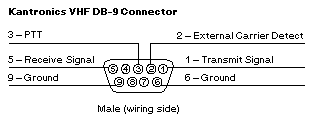
\includegraphics[width=0.75\linewidth]{images/RadioPortPinout.png} 
	\caption{Example Radio Port pin out for Kantronics, also consistent with others including OpenTrackers\,\cite{Martin2014}.}
   \label{RadioPortPinout}
\end{figure}
\begin{figure}
  \centering
	\includegraphics[width=0.75\linewidth]{images/BreakOutBoard.png} 
	\caption{Break-out board fabricated for hardware testing. There are two audio ports on the board; one for audio in and the other for audio out. On the right is the barrel jack for supplying power.}
   \label{BreakOutBoard}
\end{figure}

\section{New javAX25 Demodulator Testing Framework}
Included within the javAX25 suite was a testing application that could both generate and decode packets. However, it was limited to only being able to specify one audio file and one demodulation algorithm. Using this test file as a basis, a new testing application was created that allowed for the multiple demodulators to be compared side by side against multiple audio files with a single run of the application. In addition to the output being printed to the console, it was saved to a file. Having these features in the testing application allowed for a much more streamlined analysis of all the algorithms collectively and tuning individual algorithms. One very convenient aspect of programmatically testing is that it is very easy to add a loop to try a range of tuning parameters and then look at the results to decide what is the best option. All of the results listed in the following chapter are from the testing application and mechanism described here.
